\documentclass[10pt,conference,compsocconf]{IEEEtran}

\usepackage{hyperref}
\usepackage{graphicx}	% For figure environment
\usepackage{amsmath}
%%%%%%%%%%%%%%%%%%%%%%%%%%%%%%%%%%%%%%%%%%%%%%%%%%%%%%%%%%%%%
% Some tools
% Includes a figure
% The first parameter is the label, which is also the name of the figure
%   with or without the extension (e.g., .eps, .fig, .png, .gif, etc.)
%   IF NO EXTENSION IS GIVEN, LaTeX will look for the most appropriate one.
%   This means that if a DVI (or PS) is being produced, it will look for
%   an eps. If a PDF is being produced, it will look for nearly anything
%   else (gif, jpg, png, et cetera). Because of this, when I generate figures
%   I typically generate an eps and a png to allow me the most flexibility
%   when rendering my document.
% The second parameter is the width of the figure normalized to column width
%   (e.g. 0.5 for half a column, 0.75 for 75% of the column)
% The third parameter is the caption.
\newcommand{\scalefig}[4]{
  \begin{figure}[ht!]
    % Requires \usepackage{graphicx}
    \centering
    \includegraphics[width=#2\columnwidth]{pics/#1}
 \caption{#3}
    \label{#4}
  \end{figure}}
  
  \newcommand{\doublefig}[5]{
  \begin{figure}[ht!]
    % Requires \usepackage{graphicx}
    \centering
    \includegraphics[width=#3\columnwidth]{../pics/#1}\hfill
    \includegraphics[width=#3\columnwidth]{../pics/#2}
 \caption{#4}
    \label{#5}
  \end{figure}}

% \mathbf
\newcommand{\m}[1]{\mathbf{#1}}
\newcommand{\xx}{\mathbf{x}}
\newcommand{\xt}{\mathbf{x}^T}
\newcommand{\yy}{\mathbf{y}}
\newcommand{\ww}{\mathbf{w}}
\newcommand{\XX}{\mathbf{X}}
 
\newcommand{\Lagr}{\mathcal{L}}
\newcommand{\Lmse}{\Lagr_{MSE}}

% argmin
\newcommand{\argmin}[1]{\underset{#1}{\operatorname{argmin}}}
\newcommand{\argmax}[1]{\underset{#1}{\operatorname{argmax}}}
\newcommand{\mmin}[1]{\underset{#1}{\operatorname{min}}}
\newcommand{\mmax}[1]{\underset{#1}{\operatorname{max}}}

\newcommand*\colvec[3][]{
    \begin{pmatrix}\ifx\relax#1\relax\else#1\\\fi#2\\#3\end{pmatrix}
}


\begin{document}
\title{Project 2: Road Segmentation}

\author{
  Team Bazinga:
  Gael Moccand, Pascal Bienz\\
  gael.moccand@gmail.com, pascal.bienz@gmail.com\\
  \textit{Machine Learning Course, EPFL}
}

\maketitle

\begin{abstract}
In this work we present two methods to segment roads on satellite images. We first show how we can augment an image dataset when the one at disposal is too small to properly train a machine learning algorithm. Then we quickly demonstrate what features can be exploited and how to handle them in order to make the best prediction with a linear logistic regression. Finally, we present a method based on a deep fully convolutional neural network architecture for semantic pixel-wise segmentation called SegNet.
\end{abstract}

\section{Introduction}
The goal of this work is to segment roads on satellite images (Figure \ref{fig:satImage}) by using machine learning techniques. In other words, we want to assign a label (road or background) to each pixel of the image. Before selecting the best algorithm, an effort is made on how to augment a small image data set and how to get the most relevant features out of it. Then we present 2 different classes of algorithm. The first one is a linear logistic regression whereas the second one, called SegNet~\cite{segnet} uses a more complicated scheme based on a convolutional neural network (CNN).\\

\scalefig{satImage}{0.8}{Example of satellite image.}{fig:satImage}
\scalefig{satImage_gt}{0.8}{Ground truth of satellite image example.}{fig:satImage_gt}

A set of $N = 100$ training images of size $400 \times 400$ pixels is provided. The set contains different aerial pictures of urban areas. Together with this training set, the corresponding ground truth grayscale images (Figure \ref{fig:satImage_gt}) are also available. Note that the ground truth images need to be converted into label images. Concretely, each pixel $y_i$ can only take one of the two possible values corresponding to the classes: road label $(y_i=1)$ or background label $(y_i=0)$. In order to binarize the ground truth images, a threshold of 25\% is set. This means that every pixel with an intensity lower than 75\% of the maximum possible value is set to 0 and the rest is set to 1. With 8 bits images, the maximum value is 255 which sets the threshold to 191. This pixel threshold has a direct impact on the width of the road label in the computed label image.\\
The problem that arises with such a small training set (100 images only) is overfitting. Moreover in order to train any convolutional neural network properly it is necessary to augment the dataset. Analysing the training set, it is obvious that it contains mainly pictures with strictly vertical and horizontal roads. For that reason, creating new images by rotating the original ones allows to increase the size of the dataset and generates data which will be useful to better train the algorithm. Specifically, we rotate each image by angles going from 5 to 355 degrees every 5 degrees (i.e. 5, 10, 15,..., 355). That way we generate a set of images with roads in every directions. In summary, for each image of the original training set, 70 images are generated using the rotations, resulting in a new training set of 7100 images. This augmented training set is then suitable for the training of the CNN. \\

\section{Methodology}
In order to gain computational efficiency, square patches can be used instead of working with every pixels (see Figure \ref{fig:prediction_patch}). This make sense because a road is never composed by a single pixel but is rather made of blocks of pixels. The smaller the patch, the longer the simulations, but the finer the prediction. It is therefore important to find a trade-off. We've found that taking patches of size $8 \times 8$ gives decent result in a reasonable time. Within each patch, the mean and the variance in the 3 channels (RGB) are computed. On top of these 6 features, we add  the computation of the histogram of oriented gradients (HOG) in 8 directions. The HOG is a descriptor used in many computer vision tasks for object detection purpose. It also consists of splitting the image in patches and gives their gradient orientation quantized by the angle and weighted by the magnitude. This makes a total of 14 features per patch. Since we have $50 \times 50 = 2500$ patches, it makes a total of 35000 features per image.\\
\scalefig{prediction_patch}{0.8}{Example of a prediction using $16 \times 16$ patches. The predicted road are in red. Each red square correspond to a patch}{fig:prediction_patch}.


The feature matrix is pretty sparse like shown on Figure \ref{fig:hist_feats}. The histogram shows a large peak of zeros followed by a decay. This decay-like shape suggests us to manipulate the features in order to get a distribution following a normal distribution. This can be obtained by taking the square root of the features and can be observed on Figure \ref{fig:hist_sqrt_feats}.
These features are fed to a simple linear logistic regression using scikit-learn.\\
\scalefig{hist_feats}{1}{Histogram of the features computed on one of the satellite image}{fig:hist_feats}\\
\scalefig{hist_sqrt_feats}{1}{Histogram of the square root of the features computed on the same image}{fig:hist_sqrt_feats}

As a second step, we use the SegNet architecture which is a deep fully convolutional neural network. The SegNet architecture consists of a sequence of non-linear processing layers (encoders) and a corresponding set of decoders followed by a pixelwise classifier. Typically, each encoder consists of one or more convolutional layers with batch normalisation and a rectified linear unit (ReLU) non-linearity, followed by non-overlapping maxpooling and sub-sampling  \cite{segnet2}. The Figure \ref{fig:segnet_arch} shows the SegNet overall architecture.\\
Segmentation problems often use spatial softmax to try to classify each pixel. The Loss $\Lagr$ used in SegNet is basically a Spatial Multinomial Cross-Entropy that runs on each pixel of the output tensor, compared to the label image.

\scalefig{segnet}{1}{SegNet architecture \cite{segnet2}.}{fig:segnet_arch}

The SegNet implementation in tensorflow is taken from the github reference code of Leonardo Araujo \cite{leo}. Two versions of SegNet are available: "connected" and "gate connected". Both versions take the output of the previous convolver and the output convolver of the corresponding Encoder part as input for the Decoder. \\

In order to apply a cross-validation, the training set is randomly split into 2 parts. 80\%  is used for training (5680 images) and 20\% (1420 images) for testing. For SegNet, we use a mini batch of 50 images. The initial learning rate is set to 0.001 with a decay every 10000 steps. Note also that the size of the image is reduced to $224 \times 224$ pixels in order to speed up the training of the neural network.\\

To compare the methods, we compute the percentage of accurate patches (first method) or pixels (second method) prediction using the test set.

\section{Results}
The first method  using the linear logistic regression has been put aside pretty quickly because even with the features transformation (taking the square root), the prediction didn't exceed 0.59 on the test set. Taking into account that prediction by flipping a coin would give 0.5, it is not a big achievement. This is probably due to the fact that the mean, variance and HOG are not sufficient to differentiate the roads from the rest of the objects. \\
Regarding SegNet, the results are way more encouraging. Indeed the prediction rate almost reaches 0.9, with both SegNet connected (0.86) and connected gate (0.87).
\scalefig{pred}{0.9}{Complex example of satellite image. There are roads in many directions and trees on the road}{fig:pred}
\scalefig{pred_label}{0.85}{Prediction of the complex example using SegNet}{fig:pred_label}

\begin{table} [htbp]
  \centering
  \begin{tabular}[c]{|l|l|}
    \hline
    Method & Prediction rate\\
    \hline
    Patch + logistic & 0.59\\
    SegNet connected & 0.86\\
    SegNet connected gate & 0.87\\
    \hline
  \end{tabular}
  \caption{Summary of prediction rate of different methods.}
  \label{tab:results}
\end{table}

\section{Discussion}
The logistic regression yields pretty disappointing results. This can be explained by the reasons given above and by the fact that using patches has a main drawback. With this method we loose the continuity of the image and thus the information of the neighbor pixels at the boundaries of the patches. For instance, since a road is continuous, there is a bigger chance that a pixel is a road if its neighbors are roads than if they are part of the background. With more time, it would be interesting to keep the same prediction method but use much more features and possibly get information on the neighbor patches. However, finding most relevant features is a tedious job. For this reason we decided to use a deep learning method instead.\\
In the case of SegNet, we were expecting higher scores but it actually overfits a bit. This can be observed on Figure \ref{fig:overfit} which shows that after 7 iterations, the spatial loss increases again. To avoid this behavior, it would be good to have a broader training set in the sense that its images do not differ much.

\scalefig{overfitting}{0.9}{Spatial loss w.r.t the epoch number. It overfits after epoch 6.}{fig:overfit}


\section{Summary}
In this work we have shown how to augment an images training using rotations. Furthermore, we have presented the convolutional neural network SegNet which yields a fairly good prediction for road segmentation on satellite images. However, one must pay attention to overfitting very carefully.

%\begin{figure}[tbp]
%  \centering
%  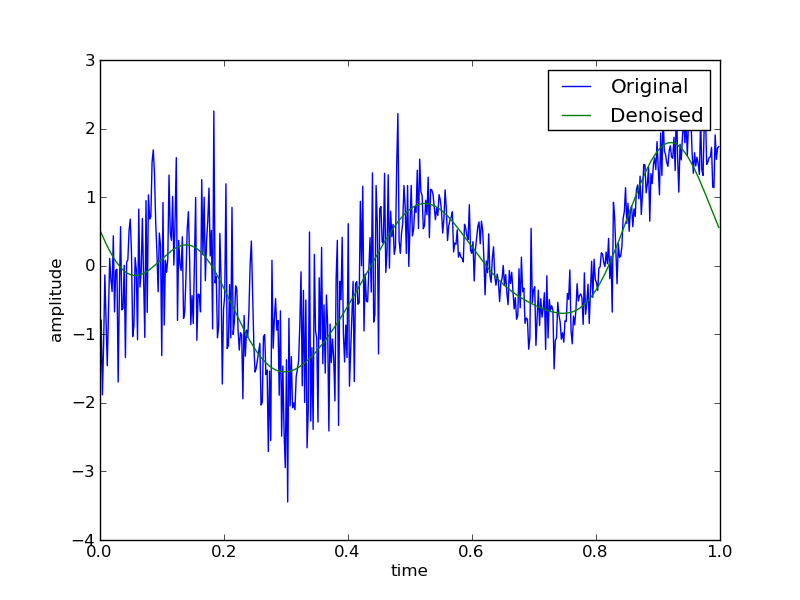
\includegraphics[width=\columnwidth]{denoised_signal_1d}
%  \caption{Signal compression and denoising using the Fourier basis.}
%  \vspace{-3mm}
%  \label{fig:denoise-fourier}
%\end{figure}
%\begin{figure}[htbp]
%  \centering
%  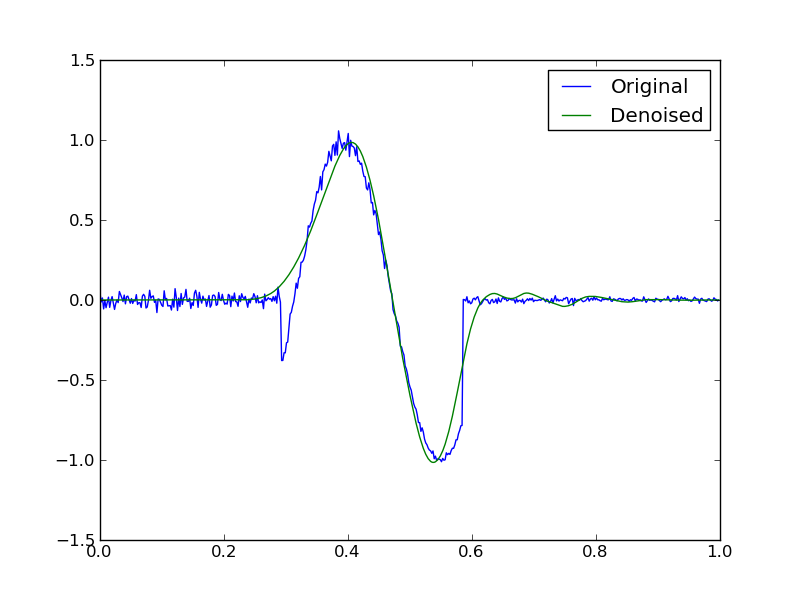
\includegraphics[width=\columnwidth]{local_wdenoised_1d}
%  \vspace{-3mm}
%  \caption{Signal compression and denoising using the Daubechies wavelet basis.}
%  \label{fig:denoise-wavelet}
%\end{figure}


\bibliographystyle{IEEEtran}
\bibliography{bazinga-literature}

\end{document}
